%\documentclass[letter]{article}
\documentclass[letter,12pt]{article}
\usepackage[letterpaper,right=1.25in,left=1.25in,top=1in,bottom=1in]{geometry}
\usepackage{setspace}

\usepackage{hyperref}
\usepackage{url}
\usepackage[pdftex]{graphicx}
\usepackage[longnamesfirst, sort]{natbib}\bibpunct[]{(}{)}{,}{a}{}{;}
\usepackage{arydshln}
\usepackage{amsmath}

%\usepackage{rotating}
%\usepackage{pdflscape}

\newcommand{\mc}{\multicolumn}

\graphicspath{{../graphs/}}

\begin{document}

\title{Transparency, Automated Redistricting,  and Partisan Strategic Interaction: \\ 
       The Case of Mexico\thanks{Paper prepared for delivery at the Annual Meeting of the American Political Science Association, Washington, DC, August 2014. We thank the Federal Electoral Institute (IFE) and the Federal Voter Registry (RFE). Special thanks to IFE's Cartography Department for sharing their experience with automated redistricting since 1996 and most of the data we analyze. We also acknowledge the support from the Asociaci\'on Mexicana de Cultura A.C.\ and CONACYT for this work.}}
% testing
\author{Alejandro Trelles {\small \url{lat44@pitt.edu}} \\
        Micah Altman {\small \url{escience@mit.edu}} \\
        Eric Magar {\small \url{emagar@itam.mx}} \\  
        Michael McDonald {\small \url{michael.mcdonald@ufl.edu}}
      }
\date{\today}
\maketitle


\begin{abstract}
%Abstract Version 1 
\noindent In the U.S.\ redistricting is deeply politicized and often synonymous with gerrymandering ---the manipulation of boundaries to promote the goals of parties, incumbents, and racial groups. In contrast, Mexico's federal redistricting has been implemented nationwide since 1996 through automated algorithms devised by the electoral management body (EMB) in consultation with political parties. In this setting, parties interact strategically and generate counterproposals to the algorithmically generated plans in a closed-door process that is not revealed outside the bureaucracy. The way that redistricting has played out so far in Mexico raises a number of questions: Were the plans produced algorithmically, in fact, optimal with respect to the selected criteria? How did partisan counterproposals differ from the bureaucratic solution? What influence did parties have on the final plan? Can automated and partisan interactive  models  generate relatively fair and unbiased plans?  We address these questions by analyzing a novel dataset that has never been available outside of the EMB and that comprises the entire set of plans proposed by political parties during the 2013 redistricting process.  Our analysis offers a unique insight into the internal workings of a purportedly autonomous EMB and the partisan effects of automated redistricting on representation.

\end{abstract}

% Comment [Eric]: Possible argument for the presentation.
% Expert committees can remove partisan bias from redistricting.
% Mexico's process allows parties to respond. Offers leverage to infer party preferences and degree of influence. 
% Analysis of party bias and responsiveness informs this, directly. 

\onehalfspacing

A fundamental principle of democratic governance is that the will of the people is the main engine of public policy. Usually, electoral institutions serve the purpose of translating the peoples' will, expressed by their votes, into the selection of representatives, who enact policies. In redistricting --- the periodic drawing of electoral boundaries, ostensibly to achieve seemingly apolitical goals such as balancing districts' populations --- the causal chain can be reversed. The drawing of new electoral boundaries may allocate voters to districts in ways that affect the number of legislative seats parties are expected to win, the careers of incumbents, and representation for racial and other interest groups. With so much at stake, scholars have found the redistricting process can distort representation, through an eponymous strategy known as gerrymandering \citep{mayhew1974vanishingMg,cox.katz.2002,erikson1972malapportionment,engstrom2006redisttrictApsr}. 

Some state governments in the US have sought to remove the opportunity for politicians to engage in gerrymandering by shifting redistricting authority from state legislatures to commissions; although some commissions' rules and membership continue to produce highly politicized outcomes, while others less so \citep{mcdonald.CommVsLegisRedistrict2004,trelles.mtz.polygob2012}. Mexicans similarly decided to overcome this challenge by delegating redistricting authority to the Federal Electoral Institute (IFE, now INE), an independent election management board created in the early 1990s. Mexico has innovated beyond the U.S.\ by employing self-tailored automated algorithms to find redistricting plans deemed optimal on \emph{a priori} criteria, and for political parties to react by offering counter-proposals \citep{trelles.mtz.polygob2012}. Here, we examine the extent to which technocrats have supplanted politicians \citep{lujambio.vives.2008} by analyzing a novel dataset describing partisan interaction within IFE in the 2013 redistricting process.

Despite that electoral officials may claim to be politically neutral, scholars find the rules by which they operate may not constrain political manipulation \citep{lijphart.1990,rossiter.etal.1997,estevez.magar.rosas.2008}. Furthermore, criteria may embody subtle second order biases that produce a predictable political outcome \citep{parker.1990}. Rather than removing political bias, redistricting by commission may perpetuate it in a different guise. In particular, IFE conducts redistricting behind closed doors, without public scrutiny, much less public participation \citep{trelles.mtz.tesisItam.2007}.\footnote{The lack of information in previous redistricting rounds, even within the IFE, generated non-functional districts. In 1997 and 2006, for instance, electoral commissioners received complains --- from several local IFE commissions and party representatives in states like Sonora and Chihuahua --- arguing that they where not allowed to participate in the redistricting process and that several districts, despite being "optimal," where splitting communities or had major geographical accidents making them dysfunctional for organizational and campaign purposes \citep{trelles.mtz.tesisItam.2007}.} The media and public are provided insufficient information to assess if the final plan embodies political mischief --- for example, how the plan produced by automation methods differs from the final plan --- before the new plan is formally adopted by IFE's Council General and takes effect \citep{trelles.datosabiertos.2015}.

% ''''' Comment [Alejandro]: Eric, could you please add to our reference list "citep{trelles.datosabiertos.2015" as follows: Trelles, Alejandro, Micah Altman, Eric Magar and Michael McDonald. 2015. Datos abiertos, representaci�n pol�tica y redistritaci�n en M�xico.  Working Paper. University of Pittsburgh. Available at SSRN.

In 2015, as in 1997 and 2006, IFE employed an algorithmic redistricting process based upon criteria agreed amongst IFE's electoral commissioners before plans were drawn. IFE used the 2005 algorithm (a simulated annealing combinatorial optimization heuristic) with the same four input parameters (population balance, compactness, municipal integrity and traveling time), but with a slightly re-weighted overall scoring function to optimize \citep{trelles.mtz.tesisItam.2007,acuerdoife2013}. \footnote{In 1996 the algorithm was known within IFE as the "heuristic model" (it was an algorithm that aggregated \emph{secciones} from West to East and from North to South in each state balancing population and trying not to split municipal administrative divisions (traveling time, compactness and minority districts were not in the picture yet); in 2006, IFE used a simulated annealing algorithm for the first time (a heuristic with a cost function that aggregated \emph{secciones} departing from a randomly chosen seed that evaluated results under a high-low "temperature" dynamic. It was in this round (2006) where four differently weighted criteria  were introduced for the first time; In 2015, IFE decided to use again the simulated annealing algorithm and the same 4 criteria weighted slightly different. Bee hive optimization was considered by the Technical Committee, but was discarded because the cost function was not improved significantly.} As in 2006, the base geography was modified so that the algorithm could not partition minority municipalities and 25 districts where created with at least 40\% of indigenous population. 

The last redistricting process towards the 2015 election offers an opportunity to assess the robustness of Mexico's redistricting process. For the first time, IFE created a web-based map sharing tool, which allows us to analyze all redistricting plans formally introduced throughout the process. A large number of plans were produced, more than in any previous redistricting, and IFE'��s Technical Redistricting Committee enabled strategic interaction between entities by allowing them to observe counter-proposals formulated by other parties through the platform. \footnote{The idea of partisan interaction was introduced in the International Redistricting Seminar celebrated at IFE in Mexico City in November 2012. IFE had allowed parties to formulate observations in 1996 and 2005, but no interaction platform existed so that parties could observe what others were proposing. The authors of this paper introduced the idea during the presentation of the Public Mapping Project Mexico (www.publicmapping.org), an open source web based platform that allows citizens and parties to analyze redistricting scenarios, observe what other users are proposing, and formulate counterproposals in order to optimize the criteria established by the legal framework and allow the authority in charge of redistricting to automatically rank and evaluate counterproposals.} 

In the end, despite consensus within party representatives at IFE to endorse the final plan (they actively participated in the process), unexpected partisan resistance in the three major national party headquarters (PAN, PRI and PRD) stalled adoption of IFE's final plan and ushered in a set of reforms to the Mexican electoral system in early 2014. The way that redistricting has played out so far in Mexico and the last set of electoral reforms ---specially the reintroduction of legislative reelection starting in 2018 and the centralization of local congressional redistricting in a single national electoral management body (INE)--- raise a number of questions: Are the adopted redistricting criteria politically neutral? Were the plans produced algorithmically, in fact, optimal with respect to the selected criteria? How did partisan counterproposals differ from the bureaucratic solution? What influence did parties have on the final plan? Can automated and partisan interactive  models  generate relatively fair and unbiased plans?

In this work we answer these questions and assess Mexico's redistricting process in search of partisan effects on representation by inspecting data that has never been available outside of the Mexican government. It comprises the machine generated plans and two rounds of strategic counter-proposals made by political parties. In the following lines we discuss how differences across parties affected their participation in the redistricting process;  what do their choices tell us about their incentives; how was a machine-based solution affected by human interaction; and the  extent to which the process can be validated by the public given the existing levels of transparency. 

%%%%%%%%%%Working this section%%%%%%%%%%%%%%

\section{Transparency and Partisan Incentives}

as IFE invited two sets of institutional actors to participate in the process: the seven national parties represented in the National Surveillance Commission (NSC) and the same seven parties represented in each of the 32 state-based Local Surveillance Commissions (LSC).

Observations and counter-proposals took place in the first and second --- out of three --- stages of the process. Once a final scenario was produced, it was voted by the EMBs Council General.

%%%%%%%%%%Working this section%%%%%%%%%%%%%%

\section{Automated Redistricting and Party Input}

Mexico adopted a mixed-member electoral system for the lower house of Congress in 1978. In the first election, three hundred single-member districts were drawn to elect three-fourths of the chamber by plurality rule. \footnote{In order to simplify our argument, we decided to leave out of this analysis boundary delimitation for proportional representation seats. PR boundary delimitation has taken place  in 1979, 1982, 1985, 1997, and 2006 and we discuss these changes and its effects on representation in the following article: Altman, Micah, Eric Magar, Michael McDonald and Alejandro Trelles. 2015. The Effects of PR Boundary Delimitation on Representation: The Case of Mexico. Working Paper. University of pittsburgh.} That proportion fell to three-fifths since 1985, but the number of single-member districts (300) has not changed. Districts were not redrawn until 1996, coinciding with the first free and fair national election in 1997 \citep{lujambio.vives.2008,trelles.mtz.tesisItam.2007}. A third redistricting occurred in 2005, and a fourth process  took place in 2013, but was aborted. In the following lines we refer to district maps by the first year they were in use, not by the actual year they were drawn.\footnote{Despite maps were actually drawn in 1978, 1996, 2005, and 2013, we use years to name the different maps, sticking to the convention of using not the date when boundaries were actually redrawn and accepted, but that of the first election the map was (or would have been) used. Thus, there is a ``1979 map'' actually drawn in 1978, a ``1997 map'' drawn in 1996, a ``2006 map'' drawn in 2004--05, and a ``2015 map'' drawn in 2013, but never used.}
     
%We need to decide if PR BOUNDARY DELIMITATION  is going to be a third paper or part of the Bias paper "Altman, Micah, Eric Magar, Michael McDonald and Alejandro Trelles. 2015. The Effects of PR Boundary Delimitation on Representation: The Case of Mexico. Working Paper. University of pittsburgh."

The method adopted has relied on machine-assisted mapping since 1997. Details have changed, but the broad lines have not \citep{trelles.mtz.tesisItam.2007}. We describe the three major stages of the redistricting process: the apportionment of seats to states; the design of an optimization algorithm; and the strategic assessment of computer-generated district blueprints by a technocrats with active, but limited involvement of political parties. 

\textbf{Apportionment}. This stage redistributes a fixed number of seats among the 32 states.\footnote{The Federal District, where Mexico City resides, is not a state proper, but is treated as one for the purpose of apportionment and redistricting.} Restrictions, reminiscent of the U.S., apply: no state may have fewer than two seats; the sole redistributive criterion above that minimum is state population; and no district may cross state boundaries. The next section elaborates the apportionment method used and some problems for representation. 

\textbf{Optimization}. This stage adopts a set of desiderata for a new map drawn from the base geography. The process makes marginal changes to boundaries, repeatedly reassigning geographical blocks between districts, systematically checking tradeoffs between criteria in a formal cost function, and iterating it all with different random seeds. Cost-minimizing district maps for each state are thus generated. The building blocks are more than 66 thousand \emph{secciones electorales} into which the Mexican territory is subdivided. \emph{Secciones} are analogous to U.S.\ census tracts, but somewhat bigger. Median \emph{secci\'on} population in the 2010 census was 1,280 persons, with a maximum at 79,232. Restrictions also apply: contiguity is a must, no district can have exclaves; as are guarantees for minority representation, \emph{municipios} (the lowest elected offices, similar to counties in the U.S.) with sizeable indigenous populations cannot be partitioned. 

More refined optimization algorithms have been used in each redistricting round. The algorithm described in the last paragraph, used for the 2015 map, replaced a method of simulated annealing used for the 2006 map. The most recent cost function included four criteria (and relative weights): population balance (.4), municipal boundary preservation (.3), travelling times inside the district (.2), and district compactness (.1). IFE would tolerate population deviations of up to 15\% across districts, and deviations above that threshold with proper justification. The tecnical committee made a 2015 map proposal (``scenario 1'') on July 17, 2013. 

\textbf{Assessment}. The third stage begins once the first scenario has been formally presented by IFE's technical committee --- appointed by the Council General --- and distributed to the parties. It involves two rounds where technical experts comment on the maps and political parties observe and suggest modifications to the maps.\footnote{This stage took approximately 4 months. It began in July 2013 and concluded in October 2013.} Amendments are proposed to the first scenario, and those that are adopted by the technical committee are then used as a starting point for another round of partisan observations to produce a second scenario. Parties are invited again to propose a second round of amendments and, once they have been analyzed and discussed by the technical committee again, a final plan is presented to the Council General to be formally approved.

\section{Partisan Strategic Interaction}

Political parties interact strategically with mapmakers, and other parties, and propose amendments to the computer-generated plans, but these amendments must improve the overall cost score to be considered for adoption. Table \ref{T:counterprops} summarizes the two rounds of amendments that took place in preparation for the 2015 map. The number of proposals increased significantly over previous redistricting, because IFE expanded participation to the its state offices, giving the parties two channels to deliver simultaneous counter-proposals. There were a total of 534 counterproposals made for the 2015 map (more than twice of the counterproposals made for the 1997 and 2006 maps). 236 counterproposals were made to the first scenario (157 from the LSC and 79 form the NSC) and 308 were made to the second scenario (139 by the LSC and 169 by NSC).

Parties actively challenged proposed districts, making 75 counter-proposals each on average. Although we expected that all 7 parties would behave as rational self-interest maximizers and strategically make competitive counter-proposals to the first scenario, the right-of-center PAN was, by far, the most successful. Nearly half of their 82 proposals were accepted, compared to about one-fifth for the other major parties (PRI and PRD). Amendments originated in both national (7 parties at the National Surveillance Commission) and state level (same 7 parties represented at 32 Local Surveillance Commissions).\footnote{The full set of parties represented in each committee were PAN, PRI, PRD, PT, PVEM, MC and PNA.} Activity at the amendment stage was enhanced by the adoption of an internal web-based map-sharing tool, which standardized counter-proposals and enabled parties to observe each others' amendments --- improving information for strategic behavior. The final proposal for Council General approval was presented on October 15, 2013. In the midst of a major electoral reform that took place in December that year, the Council General, driven by the pressure of the three major parties (PAN, PRI and PRD), chose not to decide before the end of the year. The 2015 midterm election, it was soon after learned, would be held with significantly outdated districts. 

% Comment [Alejandro]: The idea of "rational self-interest maximizers and strategically make competitive counterproposals to the first scenario" comes from the previous draft APSA2014Paper (available in G drive) and it is a possible path we want to explore to complement this paper or for publications in the near future...
% comment [Mike] what is the "strategic dimension"? How can we quantify it?
% comment [Eric] I have changed to better information for strategic behavior. Developing the game seems beyond this paper, but may shed interesting results.
% Comment [Alejandro]: A way to quantify and contrast the "strategic dimension": If we put computers (or students, as we did with the PMP demo of the State of Mexico with Eric's class) to play the game and minimize the cost function (departing from the first scenario) and maximize their utilities (as if they were parties), we could model and find the equilibrium under strictly rational principles / behavior. This would be our anchor to compare what happened in real circumstances to what could have happened if agents had been "more strategic". If we did that exercise, I am pretty sure that, given historical electoral results and the PRI's favorable position in most states across the country, the PRI would be the party that is more likely to make the most "efficient" counterproposals (not the PAN) in the first and second rounds of counterproposals. An alternative way to quantify and compare efficient solutions, from the party perspective, would be to try to minimize the cost function, while maximizing the vote share for each party by including a fifth variable/criteria (party vote share) to the four criteria that are already being used by IFE. What would have happened if the PRI and PRD had been as efficient as PAN in making counterproposals? Again, I suspect that given the PRIs electoral advantage across states, they would be, by far, better positioned to make the most effective counterproposals because they would give the simulated annealing algorithm a wider margin to offer more efficient (lower cost function) solutions... 

\begin{table}
\begin{center}
  \begin{tabular}{lrrr|rrr|r}
    Party & national & state  & total 1st & national& state  & total 2nd & Total \\ \hline
    PAN   & 17/22    & 2/20   & 19/42     & 17/24   & 4/16   & 21/40     & 40/82 \\
    PRI   & 0/0      & 2/28   & 2/28      & 8/30    & 6/26   & 14/56     & 16/84 \\
    PRD   & 3/27     & 2/21   & 5/48      & 5/29    & 5/18   & 10/47     & 15/95 \\
    PT    & 1/12     & 1/20   & 2/32      & 3/15    & 1/16   & 4/31      & 6/63 \\
    PVEM  & 0/0      & 1/20   & 1/20      & 7/28    & 3/17   & 10/45     & 11/65 \\
    MC    & 1/17     & 0/21   & 1/38      & 6/32    & 2/16   & 8/48      & 9/86 \\
    PNA   & 0/1      & 1/18   & 1/19      & 4/11    & 3/17   & 7/28      & 8/47 \\
    IFE   & 0/0      & 1/9    & 1/9       & 0/0     & 5/13   & 5/13      & 6/22 \\ \hline
    Total & 22/79    & 10/157 & 32/236    & 50/169  & 29/139 & 43/308    & 111/544 \\
  \end{tabular}
  \caption{Counter-proposals to the first and second scenarios at the National and Local Surveillance Committees. Denominator reports the number of counter-proposals made, numerator how many were adopted. Prepared by authors with information from the Federal Electoral Institute.}\label{T:counterprops}
\end{center}
\end{table}

% comment [Mike] changed PT total 1st from 2/32 to 2/22 and grand total from 32/236 to 32/226; likewise total PRD 12t and 2nd changed from 6/63 to 6/53 and grand grand total from 111/544 to 111/534
% comment [eric] nums below are what Mike's comment talks about. Those in the table above come straight from table in Alejandro's first draft. Was there a mistake in that table? Should Mike's amendments be recovered? 
    % Party & national & state  & total 1st & national & state  & total 2nd & Total \\ \hline
    % PAN   & 17/22    & 2/20   & 19/42     & 17/24    & 4/16   & 21/40     & 40/82 \\
    % PRI   & 0/0      & 2/28   & 2/28      & 8/30     & 6/26   & 14/56     & 16/84 \\
    % PRD   & 3/27     & 2/21   & 5/48      & 5/29     & 5/18   & 10/47     & 15/95 \\
    % PT    & 1/12     & 1/20   & 2/22      & 3/15     & 1/16   & 4/31      & 6/53 \\
    % PVEM  & 0/0      & 1/20   & 1/20      & 7/28     & 3/17   & 10/45     & 11/65 \\
    % MC    & 1/17     & 0/21   & 1/38      & 6/32     & 2/16   & 8/48      & 9/86 \\
    % PNA   & 0/1      & 1/18   & 1/19      & 4/11     & 3/17   & 7/28      & 8/47 \\
    % IFE   & 0/0      & 1/9    & 1/9       & 0/0      & 5/13   & 5/13      & 6/22 \\ \hline
    % Total & 22/79    & 10/157 & 32/236    & 50/169   & 29/139 & 43/308    & 111/534 \\


% comment [Alejandro]: changed the word proposal for scenario in Table 1 description (first line). Same thing in the paragraph bellow... SCENARIO = departing point; and PROPOSAL (or COUNTER PROPOSAL)  = a modification proposed by a party of IFE. 

We investigate how the 2015 redistricting process unfolded in Figure 1. For each of Mexico's thirty-two states we plot the overall score for each proposed redistricting plan (the value of the algorithm's cost function for the three scenarios are black points, numbered). The optimization objective is to produce a plan with the least cost, so plans with lower values are better than plans with higher values. The first scenario resulted from the optimization algorithm prior to party feedback, the second and third from party amendments. Colored points are party counteproposals to the second scenario, blue for the PAN, red for the PRI, yellow for the PRD, grey for the best offer by a minor party.\footnote{The same analysis for party reactions to the first proposal would reveal another interesting aspect of negotiation. A successful amendment in the first round sets the starting point for the optimization process towards the second round, and this might lend important proposal power. PAN was, by far, the most successful party in the first round.} Brown points represent two or more counter-proposals with equal scores, with one protruding petal for each plan. The cost function is expressed relative to the value of the second proposal. 

% comment [Alejandro]: Optimization just happens once, so I corrected the paragraph above...

%\begin{landscape}
\begin{figure}
\begin{center}
    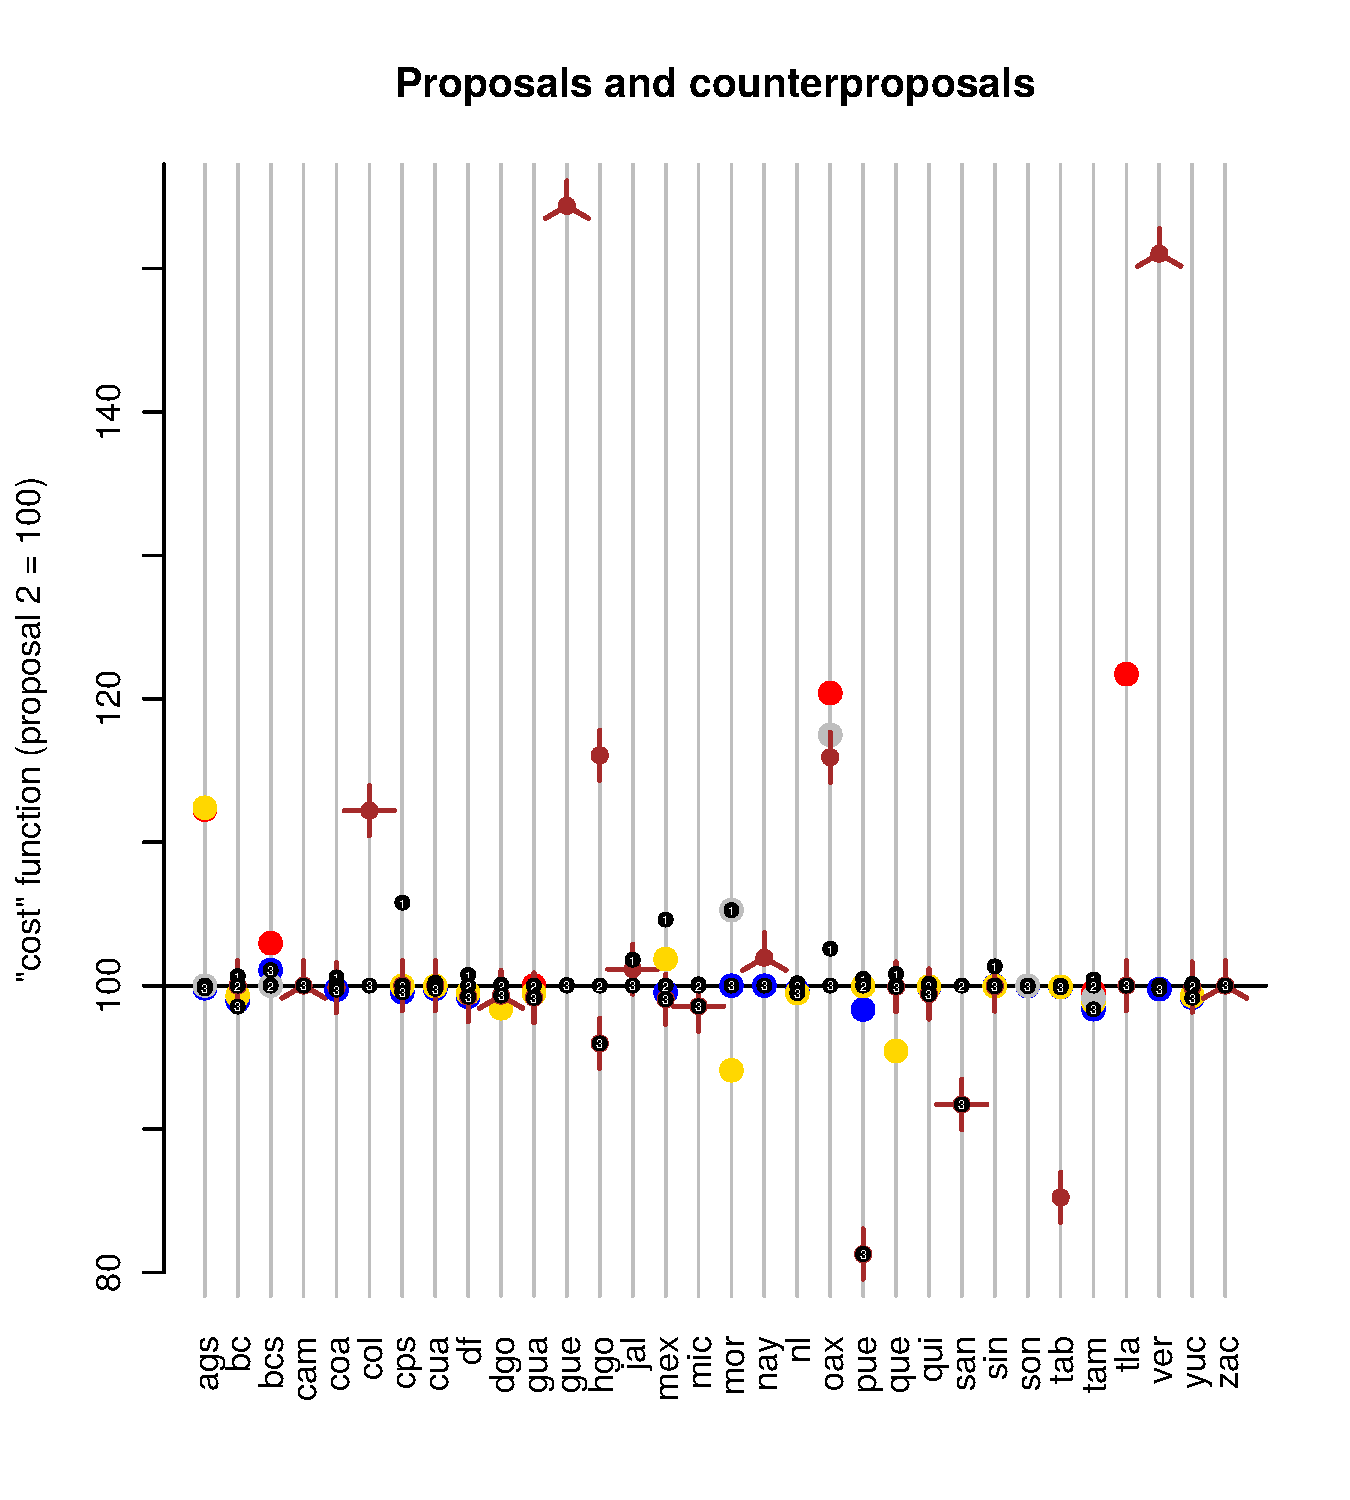
\includegraphics[width=\columnwidth]{propsAndCost.pdf} \\
  \caption{Map proposals towards 2015 by state. Black, numbered points indicate the value of the algorithm's cost function for the three map scenarios. The cost function is expressed relative to the value of the second proposal. Colored points are party counterproposals to the second proposal, blue for the PAN, red for the PRI, gold for the PRD, grey for the best offer by a minor party. Brown points report overlaps of two or more counter-proposals, one protruding petal for each overlap.}\label{F:propsAndCost}
\end{center}
\end{figure}
%\end{landscape}

In all but one state (Baja California Sur, BCS), the progression of scenarios is towards improving the cost function, as the third and final scenario has a lower score than either of the two prior scenarios. We observe numerous instances where humans "beat" the machine, by offering counter-proposals that improve the first scenario's score. These plans demonstrate how redistricting is a complex integer optimization problem where optimization algorithms can become stuck in local optima \citep{altman.mcdonald2011bard}. Where the adopted amendments to the first scenario improve the score greatly --- as is the case in Hidalgo (Hgo), Puebla (Pue) and San Luis Potos\'i (San) --- the second round of counterproposals fails to further improve the previous round given that the margin to make changes becomes narrower. We cannot know for certain if these final plans are the global optimum since the algorithm departed from a randomly chosen seed and redistricting is such a challenging optimization problem.

% comment [Mike] why did the Baja final plan score worse than the second plan? Is this a data entry error, or is something else at play?

% comment [Alejandro]: Optimization just happens once, so I corrected the paragraph above...I think there might have been something else at play, but I will definitely ask Miguel (and look at the parties comments, which we have in our G-drive). 

There are three instances where the PRD offered a counter-proposal improving upon the first scenario and all other amendments, but the amendment was rejected: Durango (Dgo), Morelos (Mor), and Quere\'taro (Que). Two identical plans proposed in Tabasco (Tab) similarly are the objectively best plans, but are rejected. In these three instances, a second round of partisan observations fails to find better plans. This provides further evidence of how automated algorithms are challenged by the complexities of redistricting. More importantly, the existence of these better plans demonstrates that politics is present in the process, likely to the detriment of the PRD.   

% comment [Mike] We should say more about the politics behind these three rejected PRD plans. Also, was the PRD one of the two parties proposing plans for Tabasco?

% comment [Eric] In Tabasco, the plans rejected were by PRI and a minor party (PVEM).

% comment [Alejandro]: We should talk about the politics behind this process in our next call and decide how we want to describe it. I can tell you my experience from 2005 and tell you about what Miguel told me of the 2013 process... In a nutshell, party representatives at IFE are not very "skilled" and they were not very efficient in terms of minimizing the cost function, while maximizing their electoral rent. They made cost winning proposals (like PAN), but where not very efficient maximizing votes. In other words, they lack expertise is big part of the explanation of inefficient outcomes. We should see them becoming more efficient in subsequent redistricting rounds (as they learn how to play this interactive game better with practice)! Most of the politics in the 2013 process was related to the apportionment stage (PRD was against redistrciting because their strong hold, Mexico City, lost a significant number of districts to the State of Mexico, a strong hold of the PRI), but it really did not have to do with things such as the criteria, how they were being wighted, the optimization algorithm or the two rounds of partisan counterproposals. I know, from very good sources, that there also was a major miss communication between party represenatatives at IFE and the parties national headquarters (this is specially true for PAN). Once the elite at the national headquarters did the math (analyzed the third scenario using electoral information), they started pressuring the General Council to postpone the approval of the plan (contrary to how their party representative was playing the game)... This explains why PAN was pressuring towards the suspension of the new map despite they won most of the counterproposals in the first and second stages.   

There are several proposals that have identical scores to the first scenario, and several instances where two proposals have identical scores. If two scenarios were tied, the technical committee would adopt the proposal that had lower cost values associated to the most relevant criteria --- population, followed by municipal integrity, traveling time and compactness at the end \citep{acuerdoife2013}. Further investigation may reveal subtle differences between these seemingly-similar plans, such as the assignment of two \emph{secciones} to different districts that has minimal changes on the overall score. We also observe numerous instances where parties propose plans that score worse than the first scenario. In many cases, as in 2005, parties decided --- even if the cost function of their counterproposal was higher than the departing scenario --- to present their plan and try to argue that their plan represented better specific communities or that responded better to geographical or socioeconomic characteristics not considered by the optimization algorithm.

% comment [Mike] when was the rule to reject worse scoring plans adopted? Was is adopted after counter-proposals to the first scenario were proposed? 

% comment [Eric] Rojano's data has lots of digits after the decimal point, so should be sensitive to seccion reaassignement. Parties must have played mostly with complete municipios, reaching the same solutions. Does this sound correct Alejandro?

% comment [Alejandro]: The answer is no Mike. This is a rule (rejecting worse scoring plans) established by the technical committee and it was socialized with all the parties prior to the creation of the first scenario (in 2005 and in 2013). This did not happen in 1996 because there was no "cost function" (for the function or for the major criteria). One of the major "improvements" in the 2005 redistricting process was that for the first time there was a score for the cost function, as well as a cost associated to each of the four criteria (population, compactness, municipal integrity and traveling time). If two scenarios were tied in the total cost function, the technical committee would have an inclination to select the proposal that had lower cost values associated to the most relevant criteria (the most important was usually the population component).  

In another key respect, all processes have remained opaque activities between electoral regulators and party representatives. New technology letting anyone interested, with little more than an Internet connection, see proposals, react, and improve them through crowd-sourcing or an open web based platform \citep{altman.mcdonald2011bard,Trelles.2015}, remains to be adopted. We observe evidence to suggest such transparency may not be welcome by all parties, as the PRD proposed objectively better plans that were never adopted.

% Comment [Alejandro]: Eric, could you please add to the citation in the paragraph above next to Altman and McDonald 2011, "Trelles Forthcoming." I understand you have them linked to Endnote, right? Thanks.

%Complete reference. Trelles, Alejandro. Forthcoming. Drawing Electoral Boundaries in Mexico: International Transparent Participative Mapping around the Globe. In The Weakest Links: Risks Arising during the Electoral Cycle, ed. Ferran  Martínez i Coma, Pippa Norris, and Richard W. Frank.  Oxford: Oxford University Press. 
% comment [Eric] DONE

% Comment [Eric]: Alejandro asked for a graph reporting proposals in terms of the cost function that IFE uses. Below is the best I could prepare... 

% comment [Mike] this graph is excellent! Thanks for producing it. I'll have to chew on it for takeaways [I've written some of this into text, but I'm keeping my original comments here]. Were these only counter-proposals to the second scenario? If proposals that would fare worse on the cost function are automatically rejected, why do we observe a fair number of proposals increasing the cost function, and presumably would be immediately rejected? (Note in bcs -- only -- the cost function increases between the second and third scenario!) Why do we see plans that improve the score rejected (mor, que, and tab)? Why do we see more than one party proposing plans with the same cost function? If these are the same plan, what is the value for more than one party proposing the same plan? Is there a way to tell if these plans are different plans, but happen to have the same score? Can we do a bias and responsiveness analysis to see if a party ever proposes a plan that works against them? I wonder if we can say something about the limits of optimization by providing the number of districts apportioned to each state. My guess is that the states with fewer plans that improve the cost function have a smaller number of districts (and thus the optimal plan is easier to discover).

% comment [Alejandro]: To answer Mike's question, I added the following text above "In many cases, as in 2005, parties decided --- even if the cost function of their counterproposal was higher than the departing scenario --- to present their plan and try to argue that their plan represented better specific communities or that responded better to geographical or socioeconomic characteristics not considered by the optimization algorithm". As I explained before, this tells us that parties are in a learning process (learning how to play this game) and sometimes they believe that arguments involving better representation could prevail over a cost function. This was extremely common in 2005, and I am sure it happened again in 2013. PRD is the party that usually has less technical resources and "skillful" personnel to defend their interests. This might explain their poor performance. The explanation of why "better cost function" plans where rejected by the committee is that there was some "margin" for the committee to evaluate if they would adopt a counterproposal. The cost function, for instance, could have improved because the traveling time was reduced, but the population balance increased slightly. In this example, the technical committee might have just decided to stay with an overall higher cost plan, but with a better population balance. This happened in 2005, and I would not be surprised if it happened again in 2013.  


\section{The 2006 Map and the 2015 Proposals}

%*** Elements of Alejandro's discussion in the APSA2014Paper of redistricting process could fit well here (file available in the G drive). ***

A new map is a full description of district boundary changes. The common way to visualize a map is by drawing it. We look at maps differently, with focus not in the physical lines and line changes but in their political consequences. Putting the 2006 map and the 2015 final proposal drawings side to side reveals boundary shifts. But unless the drawing is more data rich, assessing even the relatively simple question of how similar districts were before and after redistricting visually is a challenge. 

\begin{table}
\begin{center}
  \begin{tabular}{lrrrrr}
  Similarity between                 &   min  &  25\%  & median &  75\% &  max \\ \hline
  first 2015 proposal and status quo & 0.128  & 0.419  & 0.584  & 0.755 &  1   \\
  final 2015 proposal and status quo & 0.125  & 0.437  & 0.643  & 0.805 &  1   \\
  first and final 2015 proposals     & 0.174  & 0.705  & 0.967  & 1     &  1   \\
  \end{tabular}
  \caption{District similarity before and after the failed 2015 redistricting}\label{T:simIndex}
\end{center}
\end{table}

But a similarity index \citep[][:15--7]{cox.katz.2002} offers ground for assessment. Measurement identifies the parent district or single largest contributor of population to every new district. The $s$imilarity index divides the population that $p$arent and $n$ew district share in $c$ommon by their joint population: $s = c / (p + n - c)$. The range is zero (district shares no population at all with parent) to one (districts are identical). Table \ref{T:simIndex} describes the change that the 2015 map would have brought in the 300 single member districts, comparing IFE's initial and final proposals with the 2006 map. Also compared are the final and initial 2015 proposals themselves. 

Six percent of districts entertained no change in boundaries whatsoever vis-\`a-vis the status quo (18 districts in the initial proposal, 19 in the final), and twice as many had at least nine-tenths of the population in common (40 districts in the initial, 44 in the final proposal). Inspecting which districts were \emph{a priori} chosen for marginal or no change might reveal systematic distortions of the automated redistricting algorithm. Party feedback left 39 percent of districts in IFE's first proposal intact, and 62 percent with up from nine-tenths of the population in common. Inspecting which districts the parties targeted for major amendment --- presumably a partial reinstatement of a preferred status quo district --- should shed further light into the subject. Note how median district similarity with the 2006 map augmented from first to final proposal. So did the third quartile. Accepted counter-proposals therefore reconstituted portions of status quo districts. This seems consistent with a view where parties protect strongholds that the algorithm may have split, but further analysis must be done. 

% comment [Mike] but, the counter-proposals also improved the cost function. What this suggests is that parties will not propose amendments that do not improve their position. A straight-forward proposition, but an important one nonetheless. Still, other parties might propose plans that hurt rivals. The plans PRD plans that improved the score but were not adopted may be a smoking gun since those plans may have disrupted other parties' districts. The 6 percent of districts that had no change may be because population changes within these states are minimal and the optimal plan has already been identified in the 2006 redistricting.

% comment [Eric] Mike points to something potentially interesting for this or another paper. Could we reconstruct the counteroffers that parties made in some districts and cross that with recent electoral history in those districts?

% comment [Alejandro] Yes we could... We have all the information, right?

Noting that victory margins began widening in the mid-1960s, \citet{mayhew1974vanishingMg} saw gerrymandering as one possible explanation, incumbents influencing the preservation of safe districts. While the argument opened the heated incumbency advantage debate, the intuition may guide our inquiry. District volatility should capture a key element for analysis of map similarities. District $d$ volatility is $v_d = 1/2 \sqrt{ \sum_{p=1}^P \sum_{t=2}^3 (v_{d,p,t}- v_{d,p,t-1})^2 }$ with $p$ indexing the competing parties and $t=1,2,3$ for the 2006,  2009, and 2012 congressional elections respectively.\footnote{The measure of volatility proposed is inspired in measures of disproportionality, replacing the seats--votes difference with vote first differences. It is a squared version of a Loosemore-Hanby index \citep{loosemore.hanbyDisproportionality1971,gallagherDisproportionality1991}.} 

Mexican party strength is not proportional to the formidable entry barriers they enjoy and massive public subsidies they receive yearly \citep{magar.2007ref.2015}. Evidence of this is their inability to cultivate loyal voters. District volatility is remarkably high, as shown in Table \ref{T:volatMarginsd0}. The median district saw 25 percent of votes change party hands between 2006 and 2012 (not exactly how the index reads, but close enough). With so many volatile districts around, parties should have attempted to redress strongholds that automated redistricting split beyond recognition. How much were strongholds affected by the initial 2015 proposal? To what extent did party counter-proposals redress them? This should be a promising line of inquiry. 

\begin{table}
\begin{center}
\begin{tabular}{lrrrrr}
                    &  min.   &  25\%   & median  & 75\%   & max \\ \hline
district volatility &  .08    & .19     & .25     & .31    & .52 \\
mean PAN margin     &  $-.49$ & $-.23$  & $-.10$  & .01    & .28 \\   
mean PRI margin     &  $-.43$ & $-.09$  & $-.01$  & .07    & .28 \\   
mean PRD margin     &  $-.51$ & $-.31$  & $-.21$  & $-.04$ & .39 \\
\end{tabular}
\caption{2006 map district volatility and party margins in three congressional elections}\label{T:volatMarginsd0}
\end{center}
\end{table}

% comment [Eric] One possibility is regressing new district similarity on mean 2006--12 parent district margin, low volatility, and their interaction. Another route is the estimation of district elasticities---how vote swings in a district's \emph{secci\'ones} respond to statetwide party swings. This could provide an alternative approach to explain the district similarity index. The appendix has preliminary elasticity estimates and some discussion.



% \section{Winners and Losers}

%% comment [eric] summary of this old section might be useful

% Party effects of redistricting should involve seat swaps, to which this section turns to. Counter-factual analysis looks at how votes would have converted to seats in recent congressional elections had the 2015 map (the third scenario) been used in stead of the status quo. M\'arquez (\href{http://bit.ly/1nk4kYs}{\url{http://bit.ly/1nk4kYs}}) did this using national-level data over two decades. We proceed with state-by-state breakdowns over much a shorter span (2006, 2009, and 2012), uncovering many seat changes that cancel out in the aggregate. Compared to the status quo, counter-factual districts would slightly benefit the PRI nationwide and, by alliance, the Green party, granting them 2 to 3 extra deputies; would slightly hurt the PAN, erasing 2 to 4 victories; and would, on average, leave the left unaffected. Analysis also reveals distributive effects in nearly half the states, which complicates the assessment of partisan effects of the redistricting proposal. Counterfactuals are prepared with IFE's first and final (third) 2015 redistricting proposals, offering perspective to appreciate whether and how parties influence expert electoral regulation in general \citep{estevez.magar.rosas.2008}, and district line drawing in particular \citep{rossiter.etal.1997,cox.katz.2002}. 

% % comment [Mike] I am not certain what the counter-factual plans are. Are they the plans drawn by Eric's students? Are they the first and third scenarios for the 2015 redistricting?

% % comment [Alejandro]:The counterfactual plan/results were calculated by Eric, not his students.  Using  electoral results from Mexico's 300 SMD in 2006, 2009 and 2012, he build two counterfactual (hypothetical) scenarios: 1) Electoral results using the IFEs 2013 FIRST SCENARIO (pure optimization), and 2) Electoral results using IFEs 2013 THIRD SCENARIO (optimization + party counterporposals). 

% Column $S$ of Tables \ref{T:2006}, \ref{T:2009}, and \ref{T:2012} breaks down the federal deputy seats that parties won in the last three congressional elections by state (with actual districts). Columns $\Delta_1$ and $\Delta_3$ report seat changes had map proposals 1 and 3, respectively, been used instead. Changes are computed adding up \emph{secci\'on}-level vote returns into districts. For the sake of readability, the tables do not distinguish seats that the PRI won with the Green party (PVEM) as coalition partner.\footnote{Nine states (two in 2009, seven in 2012) combining districts with joint PRI--Green candidate and districts where each fielded a candidate complicate counterfactual computation. Most counterfactual districts in such states blend \emph{secci\'ones} with and without coalition votes, so a decision about their coalition status has to be made. I looked at whether or not coalition \emph{secci\'ones} are the most numerous in the new district, classifying it accordingly. As a consequence, several seats won in status quo districts swap from the PRI to the coalition and vice versa in mixed states' counterfactuals---mostly in the State of Mexico 2009. Keeping such swaps in the count artificially inflates the redistributive effects of redistricting.} In 2009, PRI and partner competed against each other in 237 districts while fielding joint candidates in the remaining 63, and in 2012 they competed in 101 and shared candidate in 199. Coalition in 2006 was nationwide, like that of the PRD and two minor left parties in 2006 and 2009, removing complications. 

% % pri coalition info:
% % 2009
% % 237 districts in 29 states with no coalition 
% % 63 districts in 11 states with PRI-PVEM coalition
% %  of which 46 districts in 9 states with mixed coalition status
% % 2012
% % 101 districts in 19 states with no coalition
% % 199 districts in 13 srtates with PRI-PVEM coalition
% %  of which XX in 7 states with mixed coalition status

% \begin{table}
% \begin{center}
%  \begin{tabular}{rrrr|rrr|rrr}
%       & \multicolumn{3}{c}{PAN} & \multicolumn{3}{c}{PRI coalition} & \multicolumn{3}{c}{PRD coalition} \\
% state &$S$& $\Delta_1$ &  $\Delta_3$ & $S$& $\Delta_1$ &  $\Delta_3$ & $S$& $\Delta_1$ &  $\Delta_3$  \\ \hline
% ags &   3 &     &     &      &      &      &      &      &        \\       
%  bc &   8 &     &     &      &      &      &      &      &        \\       
% bcs &     &     &     &      &      &      &    2 &      &        \\       
% cam &     &     &     &    2 &      &      &      &      &        \\       \hdashline
% coa &   5 & $-1$& $-1$&    2 &  $+1$&  $+1$&      &      &        \\       
% col &   2 &     &     &      &      &      &      &      &        \\       
% cps &     &     & $+1$&    7 &  $-1$&      &    5 &  $+2$&        \\       
% cua &   4 & $+2$&     &    5 &  $-2$&      &      &      &        \\       \hdashline
%  df &   2 &     &     &      &      &      &   25 &  $-3$&  $-3$  \\       
% dgo &   1 & $+1$& $+1$&    3 &  $-1$&  $-1$&      &      &        \\       
% gua &  14 & $+1$& $+1$&      &      &      &      &      &        \\       
% gue &     &     &     &      &      &      &    9 &      &        \\       \hdashline
% hgo &   1 &     &     &    4 &      &  $-1$&    2 &      &  $+1$  \\       
% jal &  18 & $+1$& $+1$&    1 &      &      &      &      &        \\       
% mex &  11 & $-1$&     &    6 &  $+1$&  $-1$&   23 &  $+1$&  $+2$  \\       
% mic &   4 &     &     &      &      &      &    8 &      &        \\       \hdashline
% mor &   2 &     & $-1$&    1 &  $-1$&      &    2 &  $+1$&  $+1$  \\       
% nay &     &     &     &    2 &      &      &    1 &      &        \\       
%  nl &   7 & $-1$& $-1$&    5 &  $+1$&  $+1$&      &      &        \\       
% oax &     &     &     &    2 &      &      &    9 &  $-1$&  $-1$  \\       \hdashline
% pue &  11 & $-1$& $-1$&    5 &  $-1$&      &      &  $+1$&        \\       
% que &   4 & $+1$& $+1$&      &      &      &      &      &        \\       
% qui &     &     &     &    2 &      &      &    1 &  $+1$&  $+1$  \\       
% san &   7 &     &     &      &      &      &      &      &        \\       \hdashline
% sin &   2 &     &     &    6 &  $-1$&  $-1$&      &      &        \\       
% son &   5 &     &     &    2 &      &      &      &      &        \\       
% tab &     &     &     &      &      &      &    6 &      &        \\       
% tam &   5 & $+1$& $+1$&    3 &      &      &      &      &        \\       \hdashline
% tla &   2 &     &     &      &      &      &    1 &      &        \\       
% ver &  11 & $-3$& $-5$&    6 &  $+2$&  $+4$&    4 &      &        \\       
% yuc &   4 & $-1$& $-1$&    1 &  $+1$&  $+1$&      &      &        \\       
% zac &   1 &     &     &      &      &      &    3 &      &        \\ \hline 
% tot & 134 & $-1$& $-4$&   65 &  $-1$&  $+3$&  101 &  $+2$&  $+1$  \\       
% abs &     & $15$& $16$&      &  $13$&  $11$&      &  $10$&  $9$  \\       
% \end{tabular}
% \caption{Seats won by state and counterfactual differences in 2006. Columns $\Delta_1$ and $\Delta_3$ report change in $S$eats won with proposals 1 and 3 (discussed in text), respectively. Row tot reports column sum, row abs the sum of absolute column values.}\label{T:2006}
% \end{center}
% \end{table}


% \begin{table}
% \begin{center}
% \begin{tabular}{rrrr|rrr|rrr|rrr}
%       & \multicolumn{3}{c}{PAN} & \multicolumn{3}{c}{PRI$^*$} & \multicolumn{3}{c}{PRD} & \multicolumn{3}{c}{Other} \\
% state &$S$& $\Delta_1$ &  $\Delta_3$ & $S$& $\Delta_1$ &  $\Delta_3$ & $S$& $\Delta_1$ &  $\Delta_3$ & $S$& $\Delta_1$ &  $\Delta_3$ \\ \hline
% ags &   2 &     &     &   1 &     &     &     &     &      &    &    & \\       
%  bc &   8 &     &     &     &     &     &     &     &      &    &    & \\       
% bcs &     &     &     &     &     &     &   2 &     &      &    &    & \\       
% cam &     &     &     &   2 &     &     &     &     &      &    &    & \\       \hdashline
% coa &     &     &     &   7 &     &     &     &     &      &    &    & \\       
% col &   1 &     &     &   1 &     &     &     &     &      &    &    & \\       
% cps &   4 & $+1$& $-1$&   4 &     & $+3$&   4 &     & $-1$ &    &    & \\       
% cua &   1 & $-1$& $-1$&   8 & $+1$& $+1$&     &     &      &    &    & \\       \hdashline
%  df &   6 & $-1$& $-1$&   1 &     &     &  17 & $-2$& $-2$ & 3  &    & \\       
% dgo &     &     &     &   4 &     &     &     &     &      &    &    & \\       
% gua &  13 & $+1$& $+1$&   1 &     &     &     &     &      &    &    & \\       
% gue &     &     &     &   8 &     &     &   1 &     &      &    &    & \\       \hdashline
% hgo &     &     &     &   7 &     &     &     &     &      &    &    & \\       
% jal &   9 & $+2$& $+3$&  10 & $-1$& $-2$&     &     &      &    &    & \\       
% %mex &   2 &     &     &   8 & $-3$& $-2$&     &     &      &    &    & \\       
% mex &   2 &     &     &  38 & $+1$& $+1$&     &     &      &    &    & \\       
% mic &   4 & $+1$&     &     &     &     &   8 & $-1$&      &    &    & \\      \hdashline 
% mor &     &     &     &   5 &     &     &     &     &      &    &    & \\       
% nay &   1 &     &     &   1 &     &     &   1 &     &      &    &    & \\       
%  nl &   5 & $-1$& $-1$&   7 & $+1$& $+1$&     &     &      &    &    & \\       
% oax &     &     &     &  11 & $-1$& $-1$&     &     &      &    &    & \\       \hdashline
% pue &     & $+2$& $+1$&  16 & $-3$& $-2$&     &     &      &    &    & \\       
% que &   1 & $+1$&     &   3 &     & $+1$&     &     &      &    &    & \\       
% qui &     &     &     &   3 & $+1$& $+1$&     &     &      &    &    & \\       
% san &   5 &     &     &   2 &     &     &     &     &      &    &    & \\       \hdashline
% sin &     & $+1$& $+1$&   8 & $-2$& $-2$&     &     &      &    &    & \\       
% son &   2 &     &     &   5 &     &     &     &     &      &    &    & \\       
% tab &     &     &     &   4 &     &     &   2 &     &      &    &    & \\       
% tam &     &     &     &   8 & $+1$& $+1$&     &     &      &    &    & \\       \hdashline
% tla &   3 &     &     &     &     &     &     &     &      &    &    & \\       
% ver &   4 & $-2$& $-2$&  17 & $+1$& $+1$&     &     &      &    &    & \\       
% yuc &     &     &     &   5 &     &     &     &     &      &    &    & \\       
% zac &     &     &     &     &     &     &   4 &     &      &    &    & \\ \hline 
% %tot &  71 & $+4$&     & 137 & $-6$& $-4$&  39 & $-3$& $-3$ & 3  &    & \\       
% tot &  71 & $+4$&     & 187 & $-1$& $+3$&  39 & $-3$& $-3$ & 3  &    & \\       
% abs &     & $14$& $12$&      &$13$& $17$&      & $3$&  $3$ &    &    & \\       
% % \begin{tabular}{rrrr|rrr|rrr|rrr|rrr}
% %       & \multicolumn{3}{c}{PAN} & \multicolumn{3}{c}{PRI} & \multicolumn{3}{c}{PRI coalition} & \multicolumn{3}{c}{PRD} & \multicolumn{3}{c}{Other} \\
% % state &$S$& $\Delta_1$ &  $\Delta_3$ & $S$& $\Delta_1$ &  $\Delta_3$ & $S$& $\Delta_1$ &  $\Delta_3$ & $S$& $\Delta_1$ &  $\Delta_3$ & $S$& $\Delta_1$ &  $\Delta_3$ \\ \hline
% % ags &   2 &     &     &   1 &     &     &      &      &      &     &     &      &    &    & \\       
% %  bc &   8 &     &     &     &     &     &      &      &      &     &     &      &    &    & \\       
% % bcs &     &     &     &     &     &     &      &      &      &   2 &     &      &    &    & \\       
% % cam &     &     &     &   2 &     &     &      &      &      &     &     &      &    &    & \\       \hdashline
% % coa &     &     &     &   7 &     &     &      &      &      &     &     &      &    &    & \\       
% % col &   1 &     &     &   1 &     &     &      &      &      &     &     &      &    &    & \\       
% % cps &   4 & $+1$& $-1$&     &     &     &    4 &      &  $+3$&   4 &     & $-1$ &    &    & \\       
% % cua &   1 & $-1$& $-1$&   8 & $+1$& $+1$&      &      &      &     &     &      &    &    & \\       \hdashline
% %  df &   6 & $-1$& $-1$&     &     &     &    1 &      &      &  17 & $-2$& $-2$ & 3  &    & \\       
% % dgo &     &     &     &   4 &     &     &      &      &      &     &     &      &    &    & \\       
% % gua &  13 & $+1$& $+1$&     &     &     &    1 &      &      &     &     &      &    &    & \\       
% % gue &     &     &     &   6 &     &     &    2 &      &      &   1 &     &      &    &    & \\       \hdashline
% % hgo &     &     &     &   6 &     &     &    1 &      &      &     &     &      &    &    & \\       
% % jal &   9 & $+2$& $+3$&   7 & $-1$& $-2$&    3 &      &      &     &     &      &    &    & \\       
% % %mex &   2 &     &     &   8 & $-3$& $-2$&   30 &  $+4$&  $+3$&     &     &      &    &    & \\       
% % mex &   2 &     &     &     &     &     &$38^*$&  $+1$&  $+1$&     &     &      &    &    & \\       
% % mic &   4 & $+1$&     &     &     &     &      &      &      &   8 & $-1$&      &    &    & \\      \hdashline 
% % mor &     &     &     &   5 &     &     &      &      &      &     &     &      &    &    & \\       
% % nay &   1 &     &     &   1 &     &     &      &      &      &   1 &     &      &    &    & \\       
% %  nl &   5 & $-1$& $-1$&   7 & $+1$& $+1$&      &      &      &     &     &      &    &    & \\       
% % oax &     &     &     &  11 & $-1$& $-1$&      &      &      &     &     &      &    &    & \\       \hdashline
% % pue &     & $+2$& $+1$&  15 & $-3$& $-2$&    1 &      &      &     &     &      &    &    & \\       
% % que &   1 & $+1$&     &   3 &     & $+1$&      &      &      &     &     &      &    &    & \\       
% % qui &     &     &     &   1 &     &     &    2 &  $+1$&  $+1$&     &     &      &    &    & \\       
% % san &   5 &     &     &   2 &     &     &      &      &      &     &     &      &    &    & \\       \hdashline
% % sin &     & $+1$& $+1$&   8 & $-2$& $-2$&      &      &      &     &     &      &    &    & \\       
% % son &   2 &     &     &   5 &     &     &      &      &      &     &     &      &    &    & \\       
% % tab &     &     &     &   4 &     &     &      &      &      &   2 &     &      &    &    & \\       
% % tam &     &     &     &   8 & $+1$& $+1$&      &      &      &     &     &      &    &    & \\       \hdashline
% % tla &   3 &     &     &     &     &     &      &      &      &     &     &      &    &    & \\       
% % ver &   4 & $-2$& $-2$&  17 & $+1$& $+1$&      &      &      &     &     &      &    &    & \\       
% % yuc &     &     &     &     &     &     &    5 &      &      &     &     &      &    &    & \\       
% % zac &     &     &     &     &     &     &      &      &      &   4 &     &      &    &    & \\ \hline 
% % %tot &  71 & $+4$&     & 137 & $-6$& $-4$&   50 &  $+5$&  $+7$&  39 & $-3$& $-3$ & 3  &    & \\       
% % tot &  71 & $+4$&     & 129 & $-3$& $-2$&$58^*$&  $+2$&  $+5$&  39 & $-3$& $-3$ & 3  &    & \\       
% \end{tabular}
% \caption{Seats won by state and counterfactual differences in 2009. See Table \ref{T:2006} for column and row label meanings. $^*$Includes 50 seats that the PRI won in coalition in 63 districts from 10 states.}\label{T:2009}
% % \caption{Seats won by state and counterfactual differences in 2009. See Table \ref{T:2006} for column label meanings. $^*$Includes 8 seats the PRI won solo, see text for details.}\label{T:2009} 
% \end{center}
% \end{table}


% \begin{table}
% \begin{center}
% \begin{tabular}{rrrr|rrr|rrr|rrr}
%       & \multicolumn{3}{c}{PAN} & \multicolumn{3}{c}{PRI$^*$} & \multicolumn{3}{c}{PRD coalition} & \multicolumn{3}{c}{Other} \\
% state &$S$& $\Delta_1$ &  $\Delta_3$ & $S$& $\Delta_1$ &  $\Delta_3$ & $S$& $\Delta_1$ &  $\Delta_3$ & $S$& $\Delta_1$ &  $\Delta_3$ \\ \hline
% ags &   2 & $-1$& $-1$&   1 & $+1$& $+1$&      &      &       &    &    & \\       
%  bc &   1 &     &     &   7 &     &     &      &      &       &    &    & \\       
% bcs &   2 &     &     &     &     &     &      &      &       &    &    & \\       
% cam &     &     &     &   2 &     &     &      &      &       &    &    & \\       \hdashline
% coa &   3 &     &     &   4 &     &     &      &      &       &    &    & \\       
% col &     &     &     &   2 &     &     &      &      &       &    &    & \\       
% cps &     &     &     &   9 & $+1$& $+2$&      &      &       & 3  &    & $-1$ \\       
% cua &   1 & $-1$&     &   8 & $+1$&     &      &      &       &    &    & \\       \hdashline
%  df &   1 &     &     &     &     &     &   26 &  $-3$&  $-3$ &    &    & \\       
% dgo &     &     &     &   4 &     &     &      &      &       &    &    & \\       
% gua &   7 & $+2$& $+2$&   7 & $-1$& $-1$&      &      &       &    &    & \\       
% gue &     &     &     &     &     &     &    9 &      &       &    &    & \\       \hdashline
% hgo &     &     &     &   7 &     &     &      &      &       &    &    & \\       
% jal &   1 &     &     &  18 &     &     &      &  $+1$&  $+1$ &    &    & \\       
% mex &   1 & $-1$& $-1$&  31 & $+3$& $+2$&    8 &  $-1$&       &    &    & \\       
% mic &     &     &     &   8 & $+1$&     &    4 &  $-1$&       &    &    & \\       \hdashline
% mor &     &     &     &   1 &     &     &    4 &      &       &    &    & \\       
% nay &     &     &     &   3 &     &     &      &      &       &    &    & \\       
%  nl &   6 & $-2$& $-2$&   6 & $+2$& $+2$&      &      &       &    &    & \\       
% oax &     &     &     &   1 & $-1$& $-1$&   10 &      &       &    &    & \\       \hdashline
% pue &   4 & $-1$&     &  12 & $-1$& $-2$&      &  $+1$&  $+1$ &    &    & \\       
% que &   2 & $+1$& $+1$&   2 &     &     &      &      &       &    &    & \\       
% qui &     &     &     &   2 &     &     &    1 &  $+1$&  $+1$ &    &    & \\       
% san &   2 & $+1$&     &   5 & $-1$&     &      &      &       &    &    & \\       \hdashline
% sin &   2 &     &     &   6 & $-1$& $-1$&      &      &       &    &    & \\       
% son &   5 &     &     &   2 &     &     &      &      &       &    &    & \\       
% tab &     &     &     &     &     &     &    6 &      &       &    &    & \\       
% tam &   6 & $-1$& $-1$&   2 & $+2$& $+2$&      &      &       &    &    & \\       \hdashline
% tla &     &     &     &   1 &     &     &    2 &      &       &    &    & \\       
% ver &   5 & $+1$&     &  15 & $-2$& $-1$&    1 &      &       &    &    & \\       
% yuc &   1 &     &     &   4 &     &     &      &      &       &    &    & \\       
% zac &     &     &     &   4 &     &     &      &      &       &    &    & \\ \hline
% tot &  52 & $-2$& $-2$& 174 & $+4$& $+3$&   71 &  $-2$&       & 3  &    & $-1$ \\       
% abs &     & $12$& $8$ &      &$18$& $15$&      &  $8$ &  $6$  &    &    & $2$  \\       
% % \begin{tabular}{rrrr|rrr|rrr|rrr|rrr}
% %       & \multicolumn{3}{c}{PAN} & \multicolumn{3}{c}{PRI} & \multicolumn{3}{c}{PRI coalition} & \multicolumn{3}{c}{PRD coalition} & \multicolumn{3}{c}{Other} \\
% % state &$S$& $\Delta_1$ &  $\Delta_3$ & $S$& $\Delta_1$ &  $\Delta_3$ & $S$& $\Delta_1$ &  $\Delta_3$ & $S$& $\Delta_1$ &  $\Delta_3$ & $S$& $\Delta_1$ &  $\Delta_3$ \\ \hline
% % ags &   2 & $-1$& $-1$&   1 & $+1$& $+1$&      &      &      &      &      &       &    &    & \\       
% %  bc &   1 &     &     &     &     &     &    7 &      &      &      &      &       &    &    & \\       
% % bcs &   2 &     &     &     &     &     &      &      &      &      &      &       &    &    & \\       
% % cam &     &     &     &   1 &     &     &    1 &      &      &      &      &       &    &    & \\       \hdashline
% % coa &   3 &     &     &   4 &     &     &      &      &      &      &      &       &    &    & \\       
% % col &     &     &     &     &     &     &    2 &      &      &      &      &       &    &    & \\       
% % cps &     &     &     &     &     & $+1$&    9 &  $+1$&  $+1$&      &      &       & 3  &    & $-1$ \\       
% % cua &   1 & $-1$&     &   8 & $+1$&     &      &      &      &      &      &       &    &    & \\       \hdashline
% %  df &   1 &     &     &     &     &     &      &      &      &   26 &  $-3$&  $-3$ &    &    & \\       
% % dgo &     &     &     &   4 &     &     &      &      &      &      &      &       &    &    & \\       
% % gua &   7 & $+2$& $+2$&     &     &     &    7 &  $-1$&  $-1$&      &      &       &    &    & \\       
% % gue &     &     &     &     &     &     &      &      &      &    9 &      &       &    &    & \\       \hdashline
% % hgo &     &     &     &   7 &     &     &      &      &      &      &      &       &    &    & \\       
% % jal &   1 &     &     &     &     &     &   18 &      &      &      &  $+1$&  $+1$ &    &    & \\       
% % mex &   1 & $-1$& $-1$&     &     &     &   31 &  $+3$&  $+2$&    8 &  $-1$&       &    &    & \\       
% % mic &     &     &     &   6 & $+1$&     &    2 &      &      &    4 &  $-1$&       &    &    & \\       \hdashline
% % mor &     &     &     &     &     &     &    1 &      &      &    4 &      &       &    &    & \\       
% % nay &     &     &     &   3 &     &     &      &      &      &      &      &       &    &    & \\       
% %  nl &   6 & $-2$& $-2$&     &     &     &    6 &  $+2$&  $+2$&      &      &       &    &    & \\       
% % oax &     &     &     &   1 & $-1$& $-1$&      &      &      &   10 &      &       &    &    & \\       \hdashline
% % pue &   4 & $-1$&     &   1 &     &     &   11 &  $-1$&  $-2$&      &  $+1$&  $+1$ &    &    & \\       
% % que &   2 & $+1$& $+1$&   1 &     &     &    1 &      &      &      &      &       &    &    & \\       
% % qui &     &     &     &     &     &     &    2 &      &      &    1 &  $+1$&  $+1$ &    &    & \\       
% % san &   2 & $+1$&     &   4 &     &     &    1 &  $-1$&      &      &      &       &    &    & \\       \hdashline
% % sin &   2 &     &     &   6 & $-1$& $-1$&      &      &      &      &      &       &    &    & \\       
% % son &   5 &     &     &   2 &     &     &      &      &      &      &      &       &    &    & \\       
% % tab &     &     &     &     &     &     &      &      &      &    6 &      &       &    &    & \\       
% % tam &   6 & $-1$& $-1$&   2 & $+2$& $+2$&      &      &      &      &      &       &    &    & \\       \hdashline
% % tla &     &     &     &   1 &     &     &      &      &      &    2 &      &       &    &    & \\       
% % ver &   5 & $+1$&     &     &     &     &   15 &  $-2$&  $-1$&    1 &      &       &    &    & \\       
% % yuc &   1 &     &     &     &     &     &    4 &      &      &      &      &       &    &    & \\       
% % zac &     &     &     &     &     &     &    4 &      &      &      &      &       &    &    & \\ \hline
% % tot &  52 & $-2$& $-2$&  52 & $+3$& $+2$&  122 &  $+1$&  $+1$&   71 &  $-2$&       & 3  &    & $-1$ \\       
% \end{tabular}
% \caption{Seats won by state and counterfactual differences in 2012. See Table \ref{T:2006} for column and row label meanings. $^*$Includes 122 seats that the PRI won in coalition in 199 districts from 17 states.}\label{T:2012}
% \end{center}
% \end{table}

% Seen from the national level (bottom line in each table), distributive effects are quite small. The largest drop observed is 4 seats subtracted from PAN in 2006 by the third proposal ($\Delta_3$), the largest hikes 4 extra seats for PAN in 2006 and PRI in 2009 by the first proposal ($\Delta_1$). Mean changes in the period are milder: proposal 1 returns $+\frac{1}{3}$ seat for PAN on average, $+\frac{2}{3}$ for PRI, and $-1$ for PRD; proposal 3 returns $-2$ for PAN, $+3$ for PRI, and $-\frac{2}{3}$ for the left. Adjustments made from first to final proposal are interesting. Party feedback turned the PRI from loser of one seat to winner of three in both 2006 and 2009, a net change of $\bar{\Delta_3} - \bar{\Delta_1} = 4$. Party feedback hurt the PAN almost symmetrically those years, with net changes between $-3$ and $-4$. The puzzle is that PAN had the most counter-proposals accepted (see Table \ref{T:counterprops}), which could be explained by a priority to preserve margins in strongholds and not just victories. Our analysis could presumably show this. 

% Changes nationally do not reach one percent of the full chamber. Yet putting them in contrast with recent events in the electoral arena somewhat increases their relevance. Three deputies more is one-third what the PRI--Green coalition lacks to achieve majority status in the 62nd Legislature (2012--15). And it would have sufficed to win three seats from the PRI in 2000 for the PAN to enjoy the plurality in the chamber in the 58th Legislature (2000--03). In a world of volatile voters and tight margins, characteristic of present-day Mexico, a small difference can have larger consequences. 

% National aggregates hide substantive redistricting effects at the state level. In 2006, the year most sensible to redistricting, seat distributions change in 18 states (of 32) with the proposals, but positives and negatives tend to cancel out in the national sum. The sum of absolute state changes ---the bottom row of each table--- reveals how many seat swaps (both for and against) a party experiences with redistricting. That year, the PAN, PRI and PRD would have had 16, 11, and 9 such swaps with the third redistricting proposal, respectively. These figures are between 4 and 9 times larger than national changes. In fact, the PAN's 2009 and PRD's 2012 zero nationwide changes are the sum of, respectively, 12 and 6 statewide absolute swaps that fully cancel one another. Some states by themselves involve larger distributive effects than the party's national total, as was the case of 2009 in Veracruz (PAN would get 5 seats less, PRI 4 more) and Jalisco (PAN would get 3 more seats). 

% Eleven seats would swap state party hands in 2006 with the adoption of the third proposal, four in the state of Veracruz only. This count excludes seat changes due to reapportionment---seats that one state party wins or loses with no impact on another's seats\footnote{Based on the last decade's population shifts, seven states are bound to get an extra federal seat (Chiapas, Guanajuato, Jalisco, M\'exico, Qur\'etaro, Quintana Roo, and Tamaulipas), four to lose one (Oaxaca, Puebla, Sinaloa, Veracruz) and the Federal District to lose 3.}---yet is nearly three times larger than national swaps. The ratio of state party seat swaps to national party seat swaps in 2009 and 2012 (ten and eight, respectively) remains about 3. 

% All said, inspection of counter-factuals through the lens of recent electoral history suggests that the adoption of the redistricting proposal would have helped the PRI. That party managed to redress district lines in the party ---IFE negotiations to avoid likely seat losses and get likely bonus seats instead. The regulator's decision to celebrate the 2015 midterm congressional election with outdated districts appears to postpone pain for the PAN and the left one election cycle. 


\section{Conclusion}

** To be written **

Mexico's federal districts exhibit no party bias when analyzed at the state level. Big system responsiveness, typical of first-past-the-post system in units with few federal districts, is associated with the districts. So PRI's tendency to be over-represented more than PAN and PRD, and the PRI's winning of a couple extra seats with the redistricting proposal is not the product of partisan bias. If the PRI wins more this is due to its status as the largest party in more states that the other two major parties combined. 

%Comment [Alejandro]: 

%It seems that what the above paragraph suggests is that the check and balance system (automation + partisan interaction) of Mexico's redistircting process works... A big question is if this type of model (partisan interaction, automation and openness) is something that we would like to see replicated elsewhere (i.e. US or any other country that goes through similar processes) or in the next Mexican federal or local redistricting process that will take place in the next decade... 

% We still need to analyze with closer detail the dynamic of partisan interaction and we might want to simulate what would happen with effective self-interetsed players. I assume we  we would like to understand how this interaction might develop in the near future  and its effects on representation for potential use in other countries... 

% These are some of the questiones I had in the Conclusions section of the APSA2014Paper Word Version:

% Why did parties choose to postpone the approval of the 2013-redistricting plan? Introducing legislative reelection, a higher stake for automated redistricting? Uncertainty generated by the effect of changing the boundaries in the next 4 legislative elections? Who wins and who looses by staying with the status quo (2005 maps)?  Were the adopted neutral redistricting criteria politically neutral?  Were the plans produced algorithmically, in fact, optimal with respect to the selected criteria? How did partisan counterproposals differ from the bureaucratic solution?  What influence did parties have on the final proposed plan?



\section*{Appendix} 

\subsection*{Elasticity}

% Adding more election cycles will improve the estimates. Two points now for each line as of now. 

How elastic a district is to a party's statewide (nationwide?) vote swings is interesting. Elasticity should shape redistricting preferences. A district is highly elastic for the PAN when small shifts in the party's vote statewide correspond to sharp district vote hikes. It is inelastic when it corresponds to more modest district vote changes. Negative elasticity is even conceivable, the district vote growing when the rest of the state shrinks. Local effects on mobilization and voting can move against state effects. If every \emph{secci\'on} in the district is a microcosm of the state's electorate, unit elasticity ensues. 

The measure regresses a party's three-year vote change in the \emph{secci\'on} $\Delta_s$ on the the parent state vote change $\Delta_e$ thus:  

\begin{equation}
\Delta_s = \sum\limits_{d=1}^{D_e} \alpha_d + \beta_d \Delta_e.
\end{equation}

\noindent Fixed effects for each district are considered, fitting separate $\alpha_d$ and $\beta_d$ regression coefficients for every district (indexed $d$). The model is estimated for every state separately because doing it nationwide involves too many \emph{secci\'ones} (67k) and parameters (600) for my machine. 

\begin{figure}
\begin{center}
  \begin{tabular}{cc}
    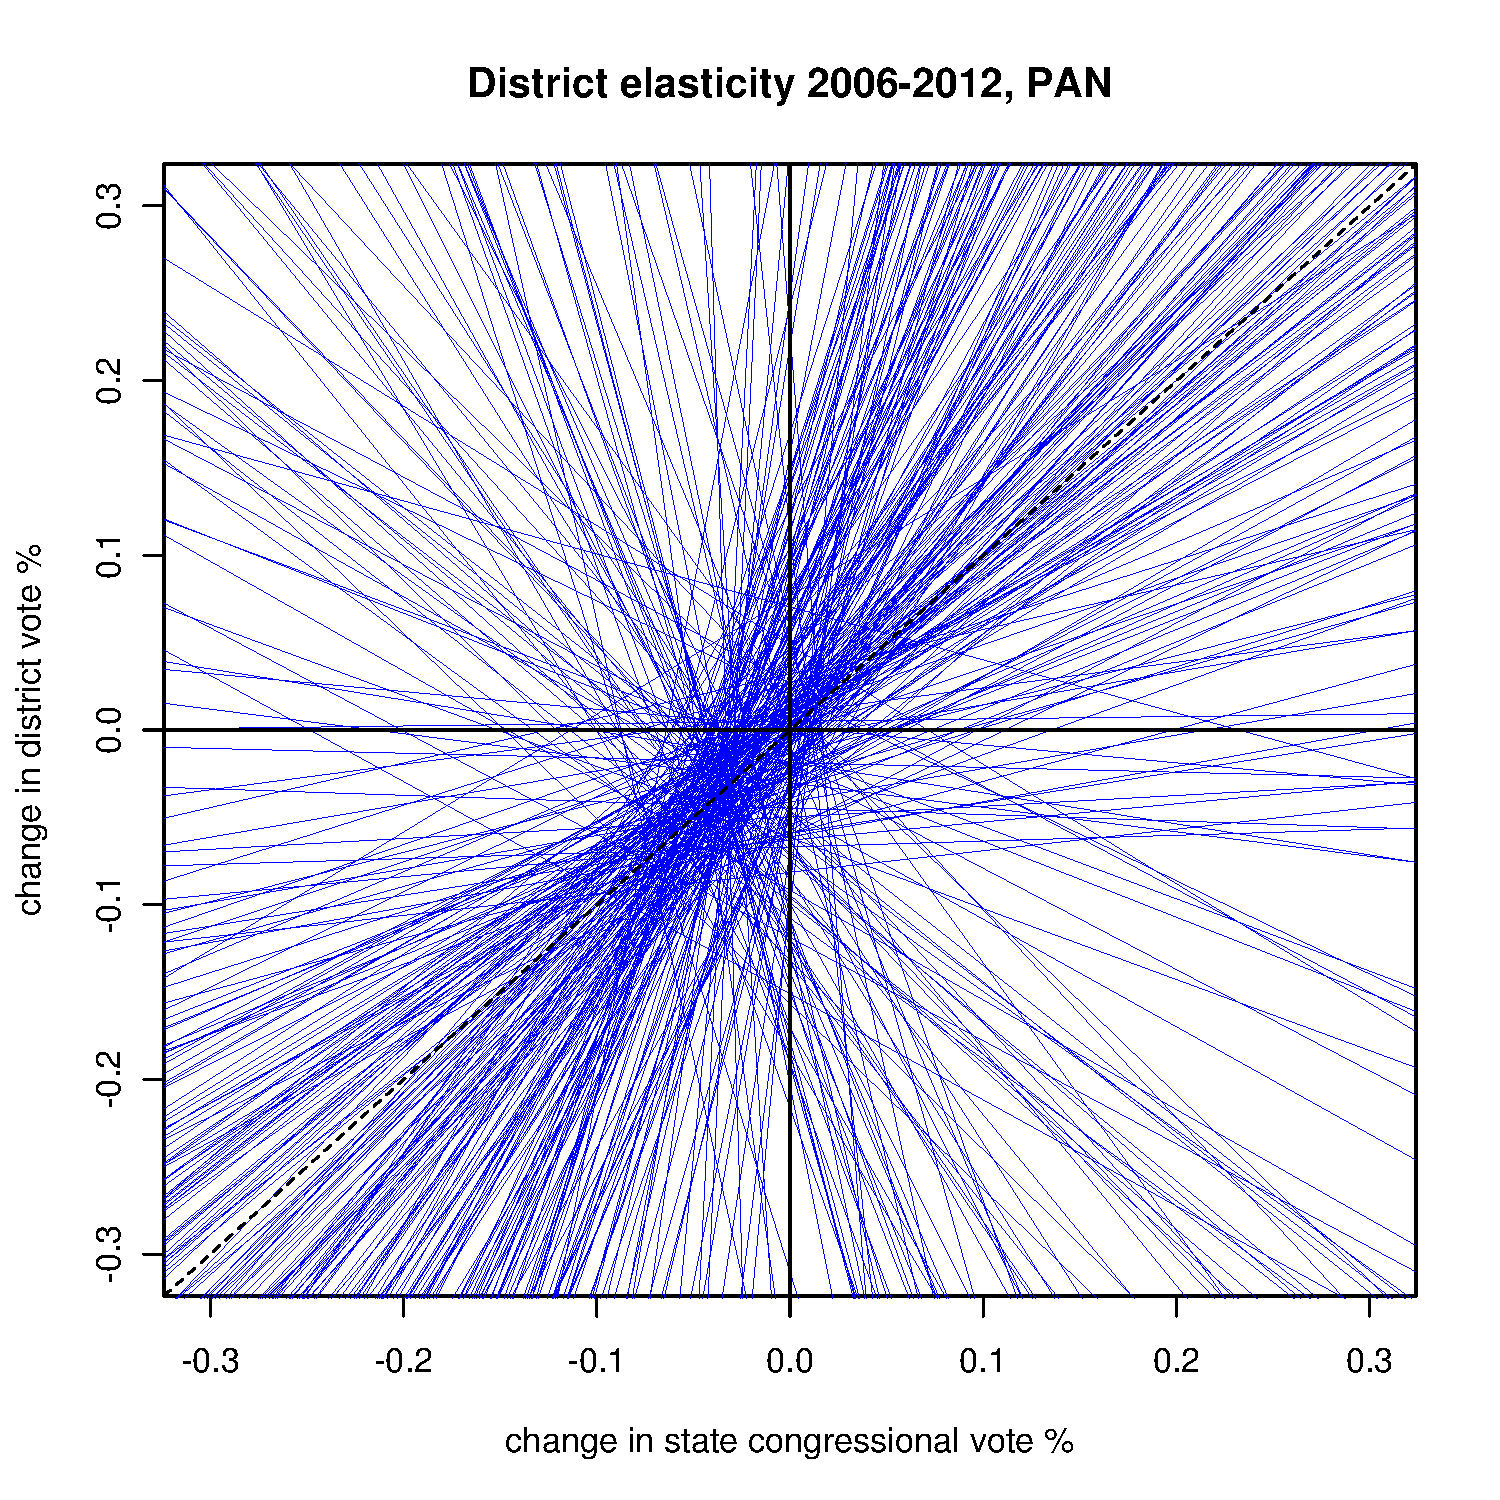
\includegraphics[width=.4\columnwidth]{elastpand0.pdf} & 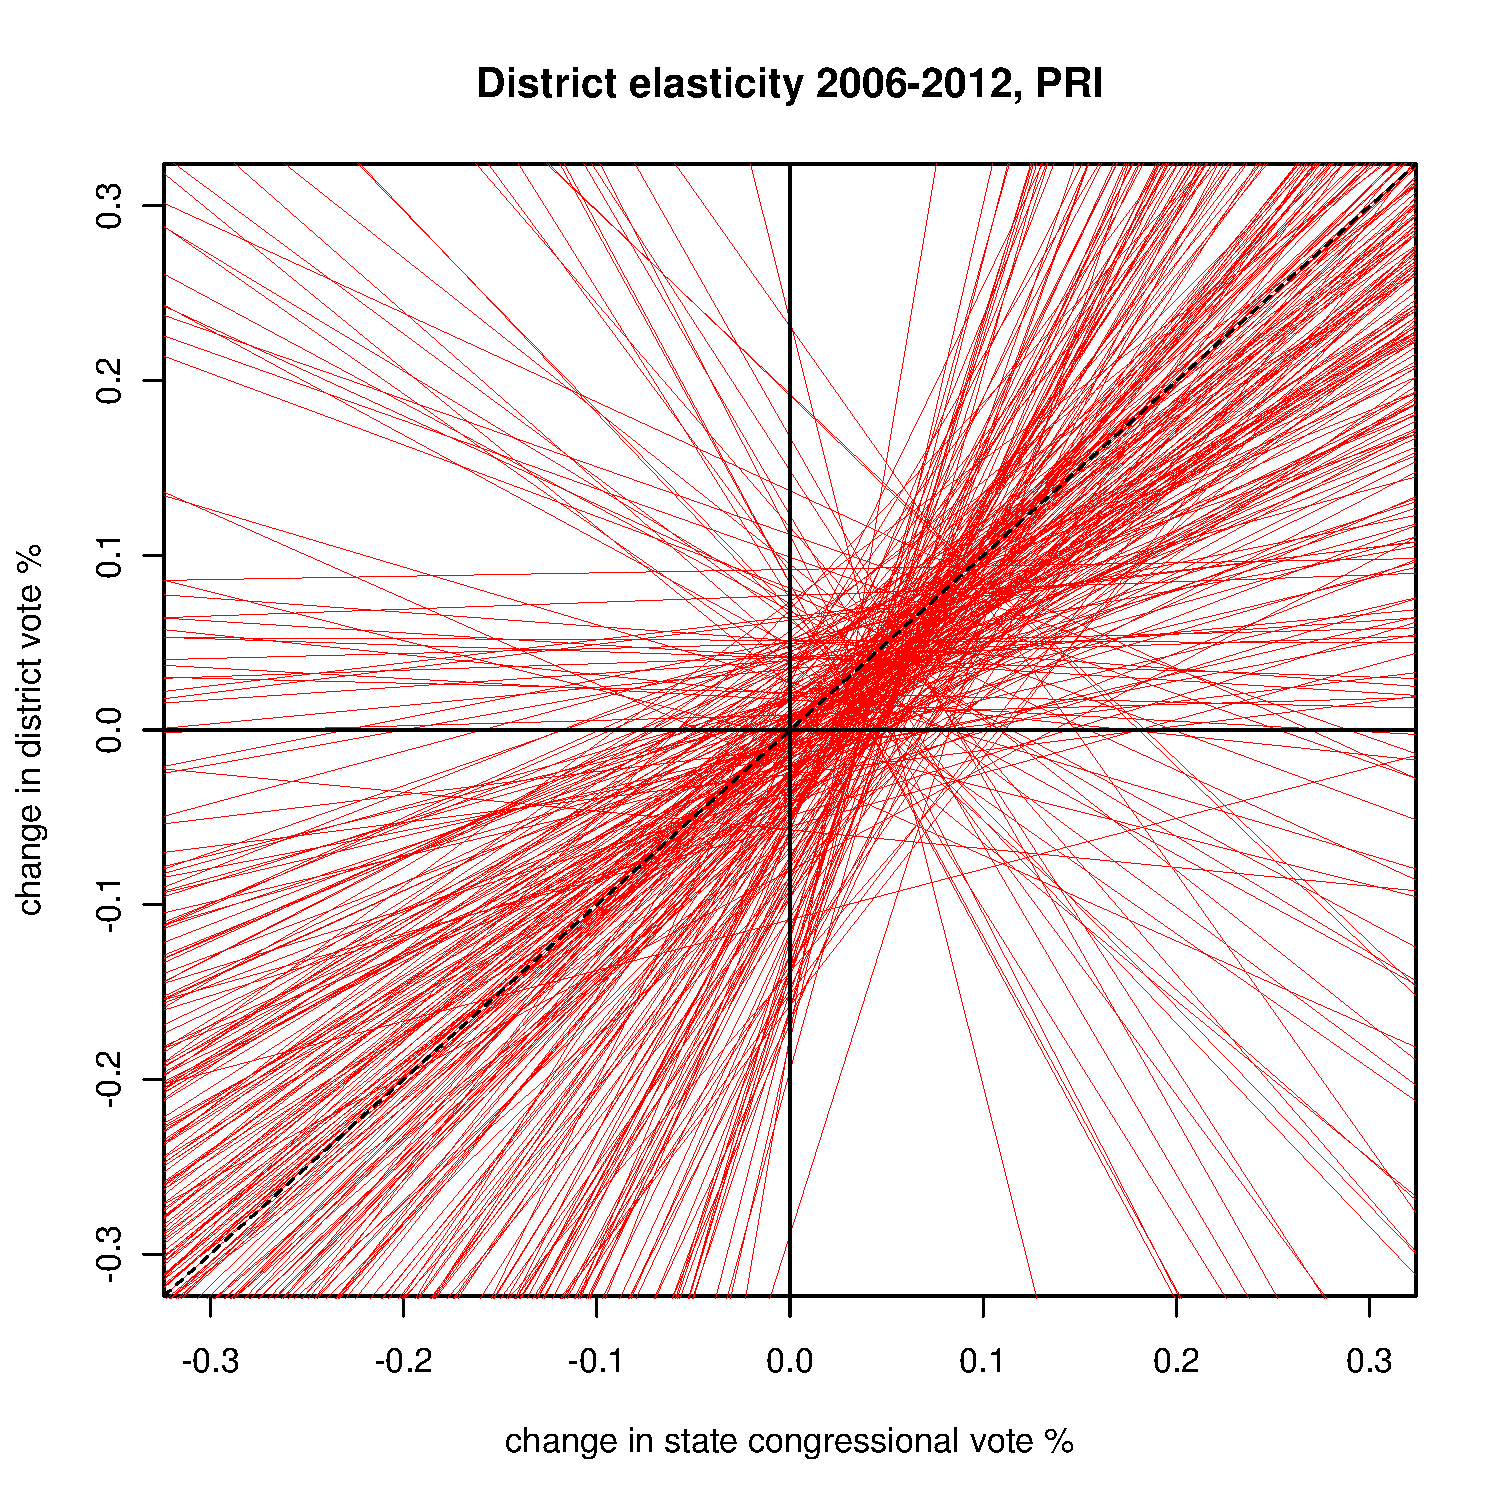
\includegraphics[width=.4\columnwidth]{elastprid0.pdf} \\
    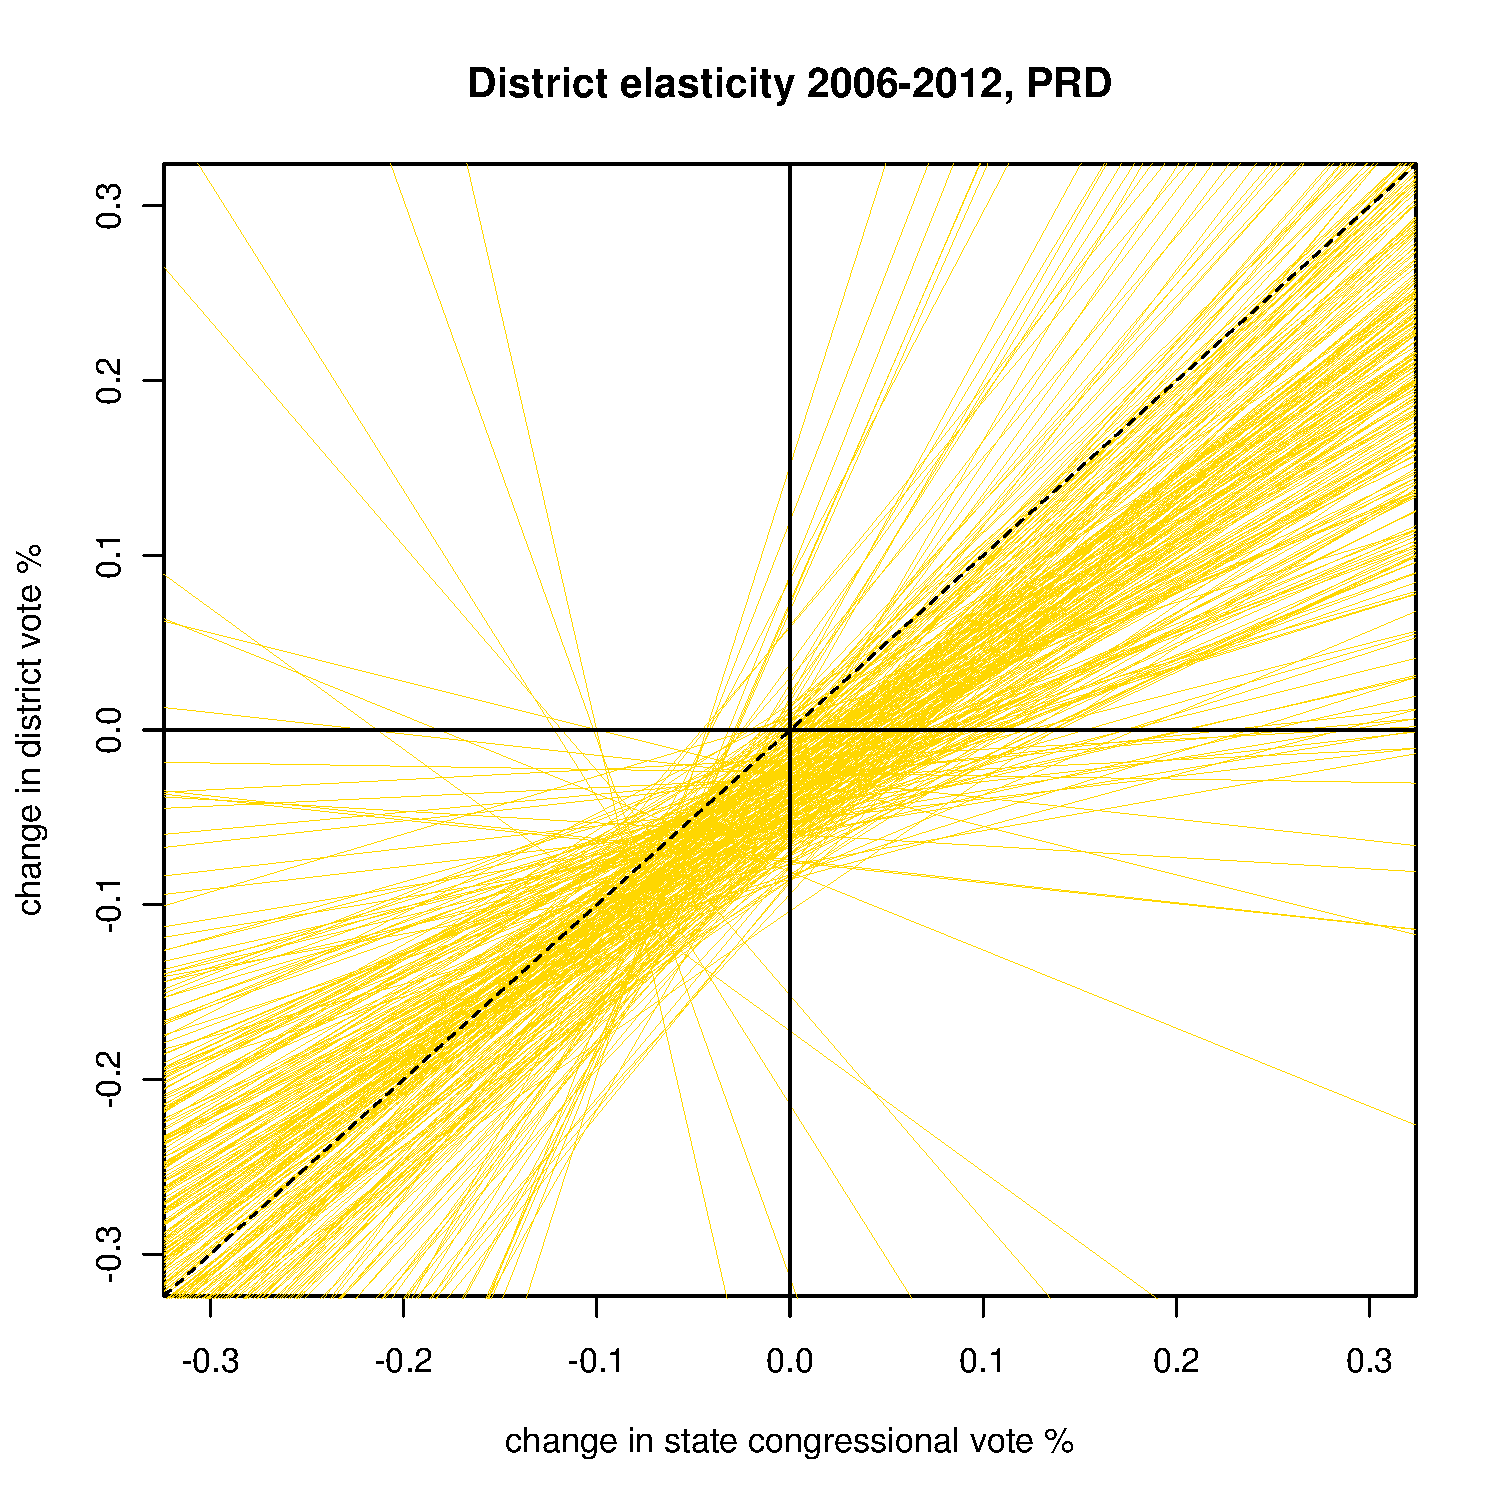
\includegraphics[width=.4\columnwidth]{elastprdd0.pdf} &  \\
  \end{tabular}
  \caption{Parties' district elasticities}\label{F:malmgnat}
\end{center}
\end{figure}



\bibliographystyle{apsr}
%\bibliography{../../../../../mydocs/magar}
\bibliography{../bib/magar}



\end{document}
